\documentclass[11pt]{article}
\pdfinfoomitdate=1
\pdftrailerid{}
\pdfsuppressptexinfo=15
\usepackage[expansion=false]{microtype}
\usepackage[margin=1.05in]{geometry}
\usepackage{amsmath,amssymb,amsthm,mathtools}
\usepackage{enumitem,booktabs,array,needspace}
\usepackage{tikz}
\usetikzlibrary{arrows.meta,positioning,calc}
\usepackage[hyphens]{url}
\usepackage[hidelinks,hypertexnames=false]{hyperref}
\usepackage[nameinlink,capitalize,noabbrev]{cleveref}
\hypersetup{pdftitle={A counterexample to Naimark's problem in ZFC},pdfauthor={OpenAI}}
\allowdisplaybreaks[1]
\numberwithin{equation}{section}
\newtheorem{theorem}{Theorem}[section]
\newtheorem{lemma}[theorem]{Lemma}
\newtheorem{proposition}[theorem]{Proposition}
\newtheorem{corollary}[theorem]{Corollary}
\theoremstyle{definition}
\newtheorem{definition}[theorem]{Definition}
\newtheorem{remark}[theorem]{Remark}
\DeclareMathOperator{\Ad}{Ad}
\DeclareMathOperator{\id}{id}
\title{A counterexample to Naimark's problem in ZFC}
\author{OpenAI}
\date{September 24, 2026}
\begin{document}
\maketitle
\begin{abstract}
We construct in ZFC a unital infinite-dimensional simple complex
$C^*$-algebra with a faithful tracial state whose nonzero irreducible
representations are all unitarily equivalent. This gives a negative answer
to Naimark's problem without additional set-theoretic assumptions.
\end{abstract}
\tableofcontents
\clearpage
\section{Introduction}
\label{sec:introduction}

For a complex Hilbert space $H$, let $K(H)$ denote the $C^*$-algebra of
compact operators on $H$. Every nonzero irreducible representation of
$K(H)$ is unitarily equivalent to its defining representation.
Naimark's problem asks whether this property characterizes the algebras
$K(H)$. We give a negative answer in ZFC.

\begin{theorem}\label{na:main}
There exists a unital infinite-dimensional simple complex $C^*$-algebra
$A$ with a faithful tracial state such that all its nonzero irreducible
representations are unitarily equivalent. In particular, $A$ is not
isomorphic to $K(H)$ for any complex Hilbert space $H$.
\end{theorem}

Here a representation is irreducible if it is nonzero and has no
nontrivial closed invariant subspace. A tracial state $\tau$ is faithful if
$\tau(a^*a)>0$ whenever $a\ne0$. The last assertion of the theorem follows
from the first: $K(H)$ is unital only when $H$ is finite-dimensional.
All algebras and Hilbert spaces in the proof are complex, and no
separability assumption is placed on $A$.

\subsection*{History and scope}
Naimark's question dates to 1951; see the historical account of the
question and Rosenberg's affirmative work in \cite{AkemannWeaver2004}.
When the unique nonzero irreducible representation acts on a separable
Hilbert space, the algebra is isomorphic to the compact operators;
see \cite[Proposition~7.2]{CalderonFarah2022}. This condition concerns
an irreducible representation, not merely a faithful representation
on a separable Hilbert space.
Akemann and Weaver constructed a counterexample
assuming Jensen's diamond principle
\cite[Theorem~5]{AkemannWeaver2004}. They also established independence
for the existence of a counterexample generated by $\aleph_1$ elements
\cite[Corollary~7]{AkemannWeaver2004}. The unrestricted existence question
does not impose this bound on the number of generators.

Subsequent work refined the set-theoretic hypotheses and the possible
structure of counterexamples. Calder\'on and Farah obtain a
counterexample from $\diamondsuit_{\mathrm{Cohen}}$ together with CH
\cite[Theorem~5.4]{CalderonFarah2022}. Under diamond, Vaccaro constructs
counterexamples whose tracial state spaces are affinely homeomorphic
to any prescribed metrizable Choquet simplex
\cite{Vaccaro2018,Vaccaro2020}. Thus the presence of a trace is already
compatible with the earlier constructions.

Tanaka gives another ZFC construction with a faithful tracial state
\cite[Theorems~1.1, 4.1 and~5.3]{Tanaka2026}, so the existence conclusion
of Theorem~\ref{na:main} is already present there. His construction
starts from the CAR algebra and uses strong shell sums and rank-one
defects. It also gives a faithful representation on a separable Hilbert
space; that representation is not irreducible. Here we give an
alternative proof organized around a selective bridge for faithfully
tracial bases without finite-dimensional irreducible representations,
reduced-HNN reordering, and dependency-closed
unique extension and countable determination. The precise hypotheses
and conclusions of these intermediate results are stated below.
Our construction has length $\mathfrak c^+$, where
$\mathfrak c=2^{\aleph_0}$; we make no assertion that this length is the
density of the resulting algebra.

\subsection*{The proof in outline}
We work with pure states, whose Gelfand--Naimark--Segal (GNS)
representations are irreducible.
Two pure states are called equivalent when their GNS representations
are unitarily equivalent. The construction repeatedly joins a chosen
pair of equivalence classes. For this procedure to be controllable,
each old pure state must have a unique state extension, and no other
pair of old classes may become equivalent.

The main analytic step starts with a faithfully tracial algebra having
no finite-dimensional irreducible representations. It adjoins a unitary
carrying one decreasing projection sequence to another. Each sequence specifies its state as
the only state taking value one on every projection; we call it a
\emph{peaking sequence}. When the two states are inequivalent and the
sequences have matching trace
values strictly decreasing to zero, the resulting reduced HNN extension
has exactly the required pure-state properties
(Theorem~\ref{na:bridge}). The extension is built from a reduced
amalgamated free product using Ueda's matrix-corner construction
\cite{UedaPreprint2008,Ueda2008}. Pure-state excision
\cite{AkemannAndersonPedersen1986} and the cross-excision estimate of
Akemann and Weaver \cite[Lemma~1]{AkemannWeaver2004} turn uniqueness
of extension and the exclusion of unintended joins into norm-decay
estimates for reduced words. The estimates apply to every old pure state.

The second step makes every pure state accessible to the recursion.
We start with a separable simple algebra, adjoin one unitary at each
active successor stage, and take norm closures of unions at limits.
Each adjunction depends on only countably many earlier generators.
If a set of generators contains all these dependencies, we prove that
every pure state on the algebra it generates has a unique extension
to the whole algebra (Theorem~\ref{na:closed-extension}). To prove this,
we postpone an omitted adjunction past the retained ones. The
no-other-join assertion of the bridge keeps its two states inequivalent
until the postponed adjunction is performed. For every pure state of
the full algebra, excision provides a separable subalgebra generated
by a countable dependency-closed set of steps on which the restriction
is pure. The closed-subiteration theorem then makes the original state
its unique extension to the full algebra
(Lemma~\ref{na:countable-determination}).

This last conclusion replaces the state-guessing role of a
set-theoretic prediction principle. At every stage below
$\mathfrak c^+$ there are at most $\mathfrak c$ pure states, so a fixed
schedule can eventually treat them all. On each separable simple
determining subalgebra, the homogeneity theorem of Kishimoto, Ozawa and
Sakai \cite{KishimotoOzawaSakai2003} supplies the next peaking sequence.
A final countable-determination argument catches every pure state of
the limit algebra.

The ingredients have several useful precedents. Akemann and Weaver
combine pure-state homogeneity with extensions joining prescribed
states \cite[Corollary~3]{AkemannWeaver2004}. Farah and Hirshberg realize prescribed countable equivalence patterns
with unique pure-state extensions
\cite[Lemma~2.3]{FarahHirshberg2017}; Vaccaro's corrected construction
combines this method with control of the trace space
\cite{Vaccaro2018,Vaccaro2020}.
Akemann, Wassermann and
Weaver prove pure-state restriction and unique-extension results for
reduced free group algebras
\cite[Proposition~2.3 and Theorem~2.6]{AkemannWassermannWeaver2010}.
Calder\'on and Farah propose using separable subalgebras that uniquely
determine the relevant states, followed by an amalgamation preserving
unique extension \cite[Section~8, especially Question~8.1]{CalderonFarah2022}.
The two features established here are the selective bridge for all
old pure states and its compatibility with dependency-closed subiterations.
Together they give the countable determination needed for the
unrestricted recursion.

Section~\ref{sec:states} proves the state-theoretic facts used below.
Section~\ref{sec:hnn} constructs the reduced adjunction, and
Section~\ref{sec:bridge} proves its pure-state properties.
Section~\ref{sec:iteration} establishes countable determination;
Section~\ref{sec:construction} carries out the final recursion.

\section{Pure states, excision, and peaking projections}\label{sec:states}

The construction must preserve unique state extensions while changing selected
equivalence classes.  This section records the state-theoretic tools for doing
so.  Its main analytic fact is excision: near the support of a pure state,
compression of an element approaches its scalar state value.

All algebras and Hilbert spaces are complex.  Unless stated otherwise, algebras
are unital and inclusions preserve the unit.  A \emph{state} on an algebra $B$
is a positive linear functional of norm one, and it is \emph{pure} if it is an
extreme point of the state space.  Write $(\pi_h,H_h,\xi_h)$ for the GNS
representation of a state $h$.  Thus $\xi_h$ is a cyclic unit vector and
$h(a)=\langle\pi_h(a)\xi_h,\xi_h\rangle$; purity is equivalent to
irreducibility of $\pi_h$.  For pure states, write $h\sim k$ when $\pi_h$ and
$\pi_k$ are unitarily equivalent.  We use
$\Ad(u)(a)=uau^*$ for conjugation by a unitary.

A \emph{tracial algebra} is a unital $C^*$-algebra equipped with a faithful
tracial state $\tau$: one has $\tau(ab)=\tau(ba)$, and $\tau(a^*a)=0$ implies
$a=0$.  Traces and other bounded functionals are extended normally to the
enveloping von Neumann algebra $B^{**}$, with the same notation.  The normal
extension of a trace is tracial, by separate ultraweak continuity.
For a representation $\pi$ of $B$, its normal extension to $B^{**}$ is
denoted by $\pi^{**}$.

For an inclusion $B\subset C$, we shall use the property
\begin{equation}\tag{U}\label{eq:U}
 \text{every pure state of $B$ has exactly one state extension to $C$.}
\end{equation}
Here uniqueness is among all states.  States always extend across a unital
inclusion, by the positive form of the Hahn--Banach theorem.

\subsection{Unique extensions and peaking}

\begin{lemma}\label{na:unique-lift}
If a pure state $h$ of $B$ has a unique state extension $\widetilde h$ to
$C\supset B$, then $\widetilde h$ is pure.
\end{lemma}
\begin{proof}
In a nontrivial convex decomposition of $\widetilde h$, both restrictions to
$B$ equal $h$ by purity.  Uniqueness then makes both states equal to
$\widetilde h$.
\end{proof}

\begin{lemma}\label{na:unitary-states}
Equivalent pure states of a unital $C^*$-algebra $B$ are conjugate by a unitary
of $B$.  Consequently, if they each have a unique state extension to an
algebra $C\supset B$, their extensions are equivalent.
\end{lemma}
\begin{proof}
Realize the two states by unit vectors $\xi,\eta$ in a common irreducible
representation $\pi$.  On their finite-dimensional span choose a unitary
carrying $\xi$ to $\eta$ and a self-adjoint logarithm of that unitary.
Kadison transitivity, including its self-adjoint form
\cite[Theorem~1]{Kadison1957}, supplies a self-adjoint $a\in B$ whose action
on this span is the chosen logarithm.  The span reduces $\pi(a)$, so
$u=e^{ia}$ satisfies $\pi(u)\xi=\eta$.  If $h$ is represented by $\xi$
and $k$ by $\eta$, then $k=h\circ\Ad(u^*)$.
Conjugating their unique extensions by the same unitary proves the last
assertion.
\end{proof}

A decreasing sequence of projections $(P_n)_{n\ge0}$ in $B$ \emph{peaks to}
a state $h$ if $h$ is the only state satisfying $h(P_n)=1$ for every $n$.
Such a state is pure: both states in any convex decomposition satisfy the
same constraints.  The following elementary observation will let us pass to
smaller algebras without assuming \eqref{eq:U} for the inclusion.

\begin{lemma}[Peaking under restriction]\label{na:peaking-restriction}
Let $B\subset C$ be a unital inclusion and let $(P_n)$ be a decreasing
sequence of projections in $B$ that peaks to a state $H$ of $C$.
Then $(P_n)$ peaks to $h=H|_B$ in $B$, and $H$ is the unique state extension
of $h$ to $C$.
\end{lemma}
\begin{proof}
Every state of $B$ satisfying the projection constraints extends to a state
of $C$ with the same constraints, hence to $H$.  It must therefore equal
$h$.  Every extension of $h$ also satisfies the constraints and must equal
$H$.
\end{proof}

\subsection{Excision and inequivalent states}

For a state $h$, its \emph{support projection} $r_h\in B^{**}$ is the least
projection on which its normal extension takes value one.  We shall prove
that this projection is minimal when $h$ is pure, together with the norm
approximation that we need. The decreasing-net form of pure-state
excision used here is proved by Akemann, Anderson, and Pedersen
\cite[Proposition~2.2]{AkemannAndersonPedersen1986}. We record a proof
in the net form used below.

\begin{lemma}[Decreasing excision]\label{na:excision}
Let $h$ be a pure state of a unital $C^*$-algebra $B$.  There is a decreasing
net of positive contractions $x_\lambda\in B$ such that $h(x_\lambda)=1$,
$x_\lambda$ decreases strongly to the minimal projection $r_h$ in $B^{**}$,
and, for every $a\in B$,
\begin{equation}\label{eq:excision}
 \|x_\lambda(a-h(a)1)x_\lambda\|\longrightarrow0.
\end{equation}
Moreover, $r_h a r_h=h(a)r_h$ for every $a\in B$.
\end{lemma}
\begin{proof}
Put
\[
 L=\{a\in B:h(a^*a)=0\},\qquad N=L\cap L^*.
\]
Here $L$ is a closed left ideal and $N$ is a $C^*$-subalgebra.  If $a\in L$,
then $a^*a\in N$, since
$h((a^*a)^2)\le\|a\|^2h(a^*a)=0$.

First, $h$ is the only state annihilating $N$.  If another state $k$
annihilates $N$, then $L$ is contained in the kernel of
$a\mapsto\pi_k(a)\xi_k$.  The map
$Q_h:B\to H_h$, $Q_h(a)=\pi_h(a)\xi_h$, is onto by one-vector Kadison
transitivity.  This assertion concerns the whole Hilbert space, even when
it is nonseparable.  Since $\ker Q_h=L$, the open mapping theorem for
$B/L\to H_h$ shows that
\[
 T\bigl(\pi_h(a)\xi_h\bigr)=\pi_k(a)\xi_k
\]
defines a bounded operator $T:H_h\to H_k$.  It intertwines the
representations.  Thus $T^*T$ is scalar by irreducibility of $\pi_h$;
its value on $\xi_h$ shows that $T^*T=1$.  Taking vector coefficients gives
$k=h$.

We next construct the decreasing net.  Order $N_+$ by the usual operator
order, a directed order, and set
\[
 e_s=1-(1+s)^{-1},\qquad x_s=1-e_s \qquad(s\in N_+).
\]
Functional calculus gives $e_s\in N$, and operator monotonicity of
inversion makes $(e_s)$ increasing.  For $b\in N$ and
$s\ge m(bb^*+b^*b)$,
\[
 \|(1-e_s)b\|^2
 \le \frac1m\|(1+s)^{-1}s(1+s)^{-1}\|
 \le\frac1{4m};
\]
the same estimate holds for $\|b(1-e_s)\|^2$.  Thus $(e_s)$ is an
approximate identity of $N$, and $h(x_s)=1$.

Let $q$ be the strong limit of $(e_s)$, the support projection of $N$.
Every normal state supported on $1-q$ annihilates $N$, and hence is $h$;
conversely, $h(1-q)=1$.  The corner $(1-q)B^{**}(1-q)$ therefore has
exactly one normal state.  Normal states separate its self-adjoint
elements, so this corner is scalar.  It follows that $1-q=r_h$ is
minimal and $x_s\downarrow r_h$.  The identity $r_har_h=h(a)r_h$ follows
by applying $h$ to this scalar corner.

Finally, let $\rho_s$ be arbitrary states of $B$.  Every weak-star cluster
point of the positive functionals
$a\mapsto\rho_s(x_sax_s)$ annihilates $N$, by the approximate-identity
estimates.  A nonzero cluster point, after normalization, is therefore
$h$.  For self-adjoint $a$, a failure of \eqref{eq:excision} would give a
subnet and norming states $\rho_s$ with a cluster point nonzero on
$a-h(a)1$, a contradiction.  Real and imaginary parts give the conclusion
for arbitrary $a$.
\end{proof}

\begin{lemma}[Projection excision]\label{na:projection-excision}
If decreasing projections $(P_n)$ in $B$ peak to $h$, then
$P_n\downarrow r_h$ strongly and
\[
 \|P_n(a-h(a)1)P_n\|\longrightarrow0\qquad(a\in B).
\]
In particular, if $h(a)=0$, then $\|P_n a P_t\|\to0$ on the product
index set.
\end{lemma}
\begin{proof}
The infimum of the $P_n$ in $B^{**}$ supports exactly one normal state,
namely $h$.  As in the preceding proof, it is the minimal projection
$r_h$.  For arbitrary states $\rho_n$, every cluster point $\psi$ of
$\rho_n(P_n\,\cdot\,P_n)$ vanishes on $1-P_m$ for each fixed $m$.
If $\psi\ne0$, its normalization satisfies every peaking constraint and
therefore equals $h$.  The same norming-state argument proves excision.
For the last assertion use nesting:
\[
 \|P_n a P_t\|\le \|P_{\min(n,t)}aP_{\min(n,t)}\|.
\qedhere
\]
\end{proof}

Excision also separates inequivalent states in norm.  We use the following
form of the cross-excision estimate of Akemann and Weaver
\cite[Lemma~1]{AkemannWeaver2004}.

\begin{lemma}[Cross-excision]\label{na:cross-excision}
Let $h\not\sim k$ be pure states of $B$, and let $(x_\lambda)$ and
$(y_\nu)$ be decreasing nets as in Lemma~\ref{na:excision}, for $h$ and
$k$ respectively.  Then, for every $a\in B$,
\begin{equation}\label{eq:cross-excision}
 \|x_\lambda a y_\nu\|\longrightarrow0
\end{equation}
on the product directed set.  Either net may be a peaking sequence of
projections.
\end{lemma}
\begin{proof}
The normal extension of $\pi_h$ annihilates $r_k$.  Otherwise a unit vector
in the range of $\pi_h^{**}(r_k)$ would represent $k$, by
$r_kar_k=k(a)r_k$.  Every nonzero vector in an irreducible representation
is cyclic, so this would imply $h\sim k$.

Consequently $h(ay_{\nu_0}a^*)\to0$ as $\nu_0$ increases.  For
$\nu\ge\nu_0$, the inequalities $y_\nu^2\le y_\nu\le y_{\nu_0}$ give
\begin{align*}
 \|x_\lambda a y_\nu\|^2
 &\le \|x_\lambda a y_{\nu_0}a^*x_\lambda\|\\
 &\le h(ay_{\nu_0}a^*)
   +\|x_\lambda(ay_{\nu_0}a^*-h(ay_{\nu_0}a^*)1)x_\lambda\|.
\end{align*}
Choose $\nu_0$ first, then use excision to choose $\lambda_0$.
This proves smallness on a rectangular tail and hence the product-net
limit.  Lemma~\ref{na:projection-excision} gives the stated projection
case.
\end{proof}

\begin{lemma}[Trace-null supports]\label{na:trace-null}
If $B$ has no finite-dimensional irreducible representations and $\tau$ is
a tracial state on $B$, then $\tau(r_h)=0$ for every pure state $h$.
\end{lemma}
\begin{proof}
The space $H_h$ is infinite-dimensional.  Choose orthonormal unit vectors
$\eta_j$ and unitaries $u_j\in B$ with $\pi_h(u_j)\xi_h=\eta_j$, as in
Lemma~\ref{na:unitary-states}.  The projections $u_jr_hu_j^*$ are
pairwise orthogonal, since
\[
 r_hu_i^*u_jr_h=h(u_i^*u_j)r_h=0\qquad(i\ne j).
\]
They all have trace $\tau(r_h)$, so $m\tau(r_h)\le1$ for every positive
integer $m$.
\end{proof}

\subsection{Expectations from peaking projections}

We now use projection excision to construct the conditional expectations
needed for the tracial extensions.  A \emph{conditional expectation}
$E:C\to B$ is a unital completely positive map fixing $B$ and satisfying
$E(b_1ab_2)=b_1E(a)b_2$ for $b_1,b_2\in B$.  It is \emph{faithful} if
$E(a^*a)=0$ implies $a=0$.

\begin{lemma}\label{na:trace-expectation}
For a unital subalgebra $B$ of a faithfully tracial algebra $(C,\tau)$,
there is at most one trace-preserving conditional expectation $C\to B$.
If one exists, it is faithful.
\end{lemma}
\begin{proof}
For such an expectation, bimodularity gives
$\tau(b^*E(a))=\tau(b^*a)$ for every $b\in B$.  Two expectations therefore
have difference $d\in B$ satisfying $\tau(d^*d)=0$, so they agree.
Faithfulness follows from $\tau(E(a^*a))=\tau(a^*a)$.
\end{proof}

\begin{lemma}\label{na:peaking-expectation}
Let $(B,\tau)$ be faithfully tracial.  Suppose decreasing projections
$(p_n)_{n\ge0}$ peak to $h$, with $p_0=1$ and trace values strictly
decreasing to zero.  Then
$D=C^*(p_n:n\ge0)$ is isomorphic to
$C(\mathbb N_0\cup\{\infty\})$, and there is a trace-preserving conditional
expectation $E:B\to D$.  Writing $d_n=p_n-p_{n+1}$ for the finite-point
atoms, it is given by
\begin{equation}\label{eq:peaking-expectation}
 E(a)(n)=\frac{\tau(d_nad_n)}{\tau(d_n)},\qquad E(a)(\infty)=h(a).
\end{equation}
\end{lemma}
\begin{proof}
The $d_n$ are nonzero orthogonal projections.  Their closed linear span is
isomorphic to $c_0(\mathbb N_0)$, and adjoining the unit gives the claimed
description of $D$.  Indeed $p_n=1-\sum_{j<n}d_j$ and $\|p_n\|=1$,
since $\tau(p_n)>0$.  Multiplying by $p_n$ shows that $1$ has distance
at least one from every linear combination of $d_0,\ldots,d_{n-1}$.

The values in \eqref{eq:peaking-expectation} define a continuous function:
by $d_n\le p_n$ and Lemma~\ref{na:projection-excision},
\[
 \left|\frac{\tau(d_nad_n)}{\tau(d_n)}-h(a)\right|
 \le \|p_n(a-h(a)1)p_n\|\longrightarrow0.
\]
Every coordinate of $E$ is a state, so $E$ is unital and completely
positive: positivity of each matrix amplification is tested pointwise
in the commutative range.  The map fixes $D$.  To check bimodularity,
an element of $D$ acts scalarly on each $d_n$; at infinity, $h|_D$ is the
evaluation character.  Cauchy--Schwarz for $h$ then gives
$h(ba)=h(b)h(a)$ and $h(ab)=h(a)h(b)$ for $b\in D$.
These coordinate identities prove bimodularity.

Finally, $\sum_n\tau(d_n)=1$ and the trace on $D$ has no mass at infinity.
Summing the finite coordinates gives $\tau(E(a))=\tau(a)$, since the
remaining trace satisfies
$|\tau(p_Na)|\le\|a\|\tau(p_N)\to0$.
\end{proof}

Unique state extensions and a faithful expectation will also preserve
simplicity, without a separate analysis of ideals in each extension.

\begin{lemma}\label{na:simple-extension}
Suppose $B\subset C$ satisfies \eqref{eq:U}, $B$ is simple, and there is a
faithful conditional expectation $E:C\to B$.  Then $C$ is simple.
\end{lemma}
\begin{proof}
Let $J$ be a proper closed two-sided ideal of $C$.  The quotient map
$q:C\to C/J$ is injective on $B$, since $B$ is simple and $q(1)\ne0$.
Every pure state $h$ of $B$ therefore extends through this quotient to a
state of $C$ annihilating $J$.  By \eqref{eq:U}, this extension is $h\circ E$.
Thus $h(E(a))=0$ for every positive $a\in J$ and every pure $h$ on $B$.
Pure states separate positive elements, so $E(a)=0$; faithfulness gives
$a=0$.  Hence $J=0$.
\end{proof}

\section{Reduced HNN adjunctions}\label{sec:hnn}

We now construct the extension that will join two pure-state classes.
The construction itself has a more general input: two trace-preserving
isomorphic subalgebras of a faithfully tracial algebra.  It adjoins a
unitary implementing the isomorphism, while prescribing the expectation
of every word in that unitary.  These prescriptions will also let us
restrict the construction to smaller bases and interchange two
adjunctions with data in the same base.

The matrix-corner construction below is the reduced HNN construction of
Ueda; see \cite[Proposition~2.2 and Remark~2.3]{UedaPreprint2008} and
\cite{Ueda2008}.  We give the details, including the faithful
representations and expectations needed later.  The corresponding
expectation and embedding results for reduced amalgamated free products
appear in \cite[Lemma~1.1 and Theorem~1.3]{BlanchardDykema2001}.

\subsection{The reduced adjunction}

Let $(A,\tau)$ be a unital $C^*$-algebra with faithful tracial state.
Fix unital subalgebras $D_1,D_2\subset A$, trace-preserving conditional
expectations $E_i:A\to D_i$, and a trace-preserving isomorphism
$\theta:D_1\to D_2$.  A word in $A$ and a unitary $v$ has the form
\begin{equation}\label{na:hnn-word}
 a_0v^{\epsilon_1}a_1\cdots v^{\epsilon_m}a_m,
 \qquad a_t\in A,\quad\epsilon_t\in\{+1,-1\}.
\end{equation}
For $m\geq1$, call it \emph{reduced} if every internal coefficient
satisfies
\begin{equation}\label{na:hnn-turns}
 \begin{cases}
 E_1(a_t)=0,&(\epsilon_t,\epsilon_{t+1})=(+1,-1),\\
 E_2(a_t)=0,&(\epsilon_t,\epsilon_{t+1})=(-1,+1).
 \end{cases}
\end{equation}
There is no condition at equal consecutive signs.

\begin{proposition}\label{na:hnn}
Let $(A,\tau)$ be a unital $C^*$-algebra with faithful tracial state,
let $D_1,D_2\subset A$ be unital subalgebras with trace-preserving
conditional expectations $E_i:A\to D_i$, and let
$\theta:D_1\to D_2$ be a trace-preserving isomorphism.  There is a
unital extension with a faithful tracial state extending $\tau$,
\[
 H(A)=C^*(A,v),\qquad vdv^*=\theta(d)\quad(d\in D_1),
\]
where $v$ is called the \emph{stable unitary}, and a trace-preserving
conditional expectation $E_A:H(A)\to A$
annihilating every nonempty reduced word
\eqref{na:hnn-word}.  Among faithfully tracial extensions generated by
$A$ and such a unitary, the relation and vanishing of the trace on
nonempty reduced words determine $H(A)$ uniquely, by an isomorphism
fixing $A$ and $v$.
\end{proposition}

We construct this adjunction as a matrix corner of an amalgamated free product.
The proof below records the module and its two compression expectations;
these will also be used in the pure-state bridge of Section~\ref{sec:bridge}.

\subsection{Construction from an amalgamated free product}

An element is \emph{centered} for a conditional expectation $E$ if it
belongs to $\ker E$.

\begin{lemma}\label{na:free-product}
Let $F$ and $G$ be unital $C^*$-algebras with faithful tracial states,
containing a common unital subalgebra $D$ on which the traces agree.
Suppose that $E_D^F:F\to D$ and $E_D^G:G\to D$ are trace-preserving
conditional expectations.  There is a unital $C^*$-algebra $Z$ generated
by faithful copies of $F$ and $G$ agreeing on $D$, with a faithful
tracial state extending both traces and faithful trace-preserving conditional
expectations
\[
 E_D:Z\longrightarrow D,
 \qquad E_F:Z\longrightarrow F,
 \qquad E_D=E_D^F\circ E_F.
\]
The map $E_D$ vanishes on every nonempty alternating product of elements
of $\ker E_D^F$ and $\ker E_D^G$.  The map $E_F$ vanishes on every product
\begin{equation}\label{na:free-core}
 a_0 b_1 a_1\cdots b_m a_m,
 \qquad m\geq1,
\end{equation}
where $a_0,a_m\in F$, $b_t\in\ker E_D^G$, and
$a_t\in\ker E_D^F$ for $0<t<m$.  The linear span of $F$ and these
products is dense in $Z$.
\end{lemma}

\begin{proof}
For $i\in\{F,G\}$, complete $i$ as a right Hilbert $D$-module $L_i$
with inner product
\[
 \langle x,y\rangle_D=E_D^i(x^*y).
\]
Left multiplication by $a\in i$ is bounded, since
\[
 E_D^i(x^*a^*ax)\leq\|a\|^2E_D^i(x^*x),
\]
and its adjoint is left multiplication by $a^*$.  The expectation gives
an orthogonal decomposition
\[
 L_i=D\oplus L_i^\circ,
 \qquad L_i^\circ=\overline{\ker E_D^i}.
\]
Both summands are invariant under left and right multiplication by $D$.
Form the Hilbert $D$-module
\begin{equation}\label{na:free-module}
 K=D\oplus
 \bigoplus_{\substack{m\geq1,\ i_t\in\{F,G\}\\i_t\ne i_{t+1}}}
 L_{i_1}^\circ\otimes_D\cdots\otimes_D L_{i_m}^\circ.
\end{equation}
Here $\otimes_D$ is the interior tensor product of Hilbert modules; the
left $D$-action on a word acts on its first factor.  The first summand
$D$ is called the vacuum summand, with distinguished vector $1$.

Let $K^{(i)}$ be the vacuum summand together with all words not starting
with $i$.  The decomposition of $L_i$ identifies
\[
 K=L_i\otimes_D K^{(i)}.
\]
Represent $i$ by left multiplication on the first tensor factor.  The
two representations agree on $D$.  They are faithful: an element $a$
annihilating the vacuum satisfies $E_D^i(a^*a)=0$, so its faithful
factor trace gives $a=0$.  Let $Z$ be the $C^*$-algebra they generate in
the adjointable operators on $K$.

A centered element of $i$ acting on $K^{(i)}$ adds its own tensor
factor at the front.  Thus a nonempty alternating centered product has
zero vacuum compression.  Centering arbitrary factor elements shows
that $D$ and these products span a dense subspace of $Z$.  Vacuum
compression consequently takes values in the left copy of $D$ and
defines the conditional expectation $E_D$.

Write $\tau_D$ for the common trace on $D$.  We next prove that
$\tau_Z=\tau_D\circ E_D$ is tracial and faithful.  For traciality,
compare $\tau_Z(aw)$ and $\tau_Z(wa)$ when $a$ belongs to one factor
and $w$ is an alternating centered word.  If $w$ has length at least
two, both values vanish.  Indeed, multiplication at a same-factor end,
followed by centering that end product, leaves either an alternating
centered word or a $D$-coefficient times a nonempty such word.  At a
different-factor end, first center $a$ and use $D$-bimodularity.  For a
one-letter word, use the factor trace when the factors agree; when they
differ, both values are zero.  For $w\in D$, use the factor trace.
Density and repeated cyclic movement of a factor now prove traciality
on all of $Z$.

Suppose $\tau_Z(z^*z)=0$.  For every $t\in Z$, traciality gives
\[
 0\leq\tau_Z(t^*z^*zt)
 =\tau_Z(ztt^*z^*)
 \leq\|t\|^2\tau_Z(zz^*)=0.
\]
The trace on $D$ is faithful, so $E_D((zt)^*(zt))=0$.  This is the
$D$-valued inner product of $zt1$ with itself, and hence $zt1=0$.  Products of
centered letters create all elementary tensors in
\eqref{na:free-module}; thus $Z1$ is dense in $K$.  It follows that
$z=0$, proving faithfulness of $\tau_Z$.

Finally, let $P_F$ be the orthogonal projection onto
$D\oplus L_F^\circ=L_F$.  This submodule reduces the $F$-action.
A core $w=b_1a_1\cdots a_{m-1}b_m$ as in
\eqref{na:free-core} sends $L_F$ into words starting with $G$, so
$P_FwP_F=0$.  Since $P_F$ commutes with $F$, arbitrary endpoint
coefficients satisfy
\[
 P_Fa_0wa_mP_F=a_0P_FwP_Fa_m=0.
\]
Successive centering shows that $F$ and the products
\eqref{na:free-core} span a dense subspace.  Their compressions belong
to the faithful left copy of $F$ on $L_F$, which is norm closed.
Compression therefore defines a conditional expectation $E_F:Z\to F$.
The vacuum lies in $L_F$, giving $E_D=E_D^F\circ E_F$ and trace
preservation.  Faithfulness follows from faithfulness of $\tau_Z$.
\end{proof}

\begin{proof}[Proof of Proposition~\ref{na:hnn}]
Take
\[
 F=M_2(A),\qquad G=M_2(D_1),\qquad D=D_1\oplus D_2.
\]
Embed $D$ in $F$ by $(d_1,d_2)\mapsto\operatorname{diag}(d_1,d_2)$
and in $G$ by
$(d_1,d_2)\mapsto\operatorname{diag}(d_1,\theta^{-1}(d_2))$.
The normalized matrix traces agree on $D$, and the maps
\[
 E_D^F(a)=(E_1(a_{11}),E_2(a_{22})),\qquad
 E_D^G(b)=(b_{11},\theta(b_{22}))
\]
are trace-preserving conditional expectations.  Apply
Lemma~\ref{na:free-product} to obtain $Z$, and retain the module
notation used in its proof.
The diagonal matrix projections $e_i=e_{ii}$ are common to the two
factors.  Set
\begin{equation}\label{na:hnn-corner}
 s=e_{21}^G,\qquad
 H(A)=e_1Ze_1,\qquad
 v=e_{12}^Fs,
\end{equation}
and identify $A$ with $e_1Fe_1$.  Then $v^*v=vv^*=e_1$.
For $d\in D_1$, the element $sds^*$ is the second-corner copy of
$\theta(d)$ in $F$, so $vdv^*=\theta(d)$ in the first corner.

The matrix units of $F$ identify $Z$ with $M_2(e_1Ze_1)$.  Under this
identification, the matrix algebra over $C^*(A,v)$ contains $F$ and
$s=e_{21}^Fv$.  It contains $G$ as well, because $G$ is generated by
$D$ and $s,s^*$.  Hence $H(A)=C^*(A,v)$.  The trace on the corner is
$2\tau_Z$, and its restriction to $A$ is $\tau$.  The restriction of
$E_F$ gives the required faithful trace-preserving expectation onto
$A$.

To check reduced words, write $q=e_{12}^F$, so $v=qs$ and
$v^*=s^*q^*$.  Between consecutive $G$-letters the internal
$F$-coefficients are
\[
\begin{array}{c|cccc}
 (\epsilon_t,\epsilon_{t+1}) &(+,+)&(+,-)&(-,+)&(-,-)\\ \hline
 \text{coefficient} &a_tq&a_t&q^*a_tq&q^*a_t.
\end{array}
\]
The first and last are off diagonal.  The middle two have zero
$D$-expectation precisely under the respective conditions in
\eqref{na:hnn-turns}.  Since $s,s^*$ are centered, the expanded word
is a product of the form \eqref{na:free-core}, and its expectation
onto $F$, hence onto $A$, is zero.

For uniqueness, split a coefficient at an opposite-sign turn as
$(a-E_i(a))+E_i(a)$.  The first term is centered at that turn, while
the second cancels two stable letters using the unitary relation.
Repeating this operation expresses every polynomial as an $A$-term
plus nonempty reduced words.  Thus the stipulated data determine the
trace of every polynomial, and in particular all moments of $x^*x$
for each polynomial $x$.

For a faithful tracial state $t$ on any $C^*$-algebra,
\begin{equation}\label{na:moment-norm}
 \|x\|=\lim_{r\to\infty}t((x^*x)^r)^{1/(2r)}.
\end{equation}
To see this, restrict $t$ to the commutative algebra generated by
$x^*x$ and the unit.  Its spectral measure has full support, by
faithfulness, and its $r$th-root moments tend to the spectral maximum.
Consequently identical polynomial trace moments give identical
polynomial norms.  The generator correspondence is therefore
isometric and extends to the asserted isomorphism.  This argument
requires no expectation in the comparison extension beyond the stated
trace-vanishing rule.
\end{proof}

We will also use the explicit spanning description of the matrix
algebra $Z$.  In the model \eqref{na:hnn-corner}, every centered
$G$-element is a sum of $D$-multiples of $s$ and $s^*$.  Absorb these
$D$-coefficients into neighboring $F$-coefficients; their internal
centering is preserved by bimodularity.  Thus $F$ and the products
\begin{equation}\label{na:matrix-word-span}
 a_0b_1a_1\cdots b_ma_m,
 \quad m\geq1,\quad b_t\in\{s,s^*\},\quad a_t\in F,
 \quad E_D^F(a_t)=0\ (0<t<m)
\end{equation}
have dense linear span in $Z$.

\begin{corollary}\label{na:hnn-restriction}
With the hypotheses of Proposition~\ref{na:hnn}, let $A'\subset A$
be a unital subalgebra containing $D_1$ and $D_2$.  Then
$C^*(A',v)\subset H(A)$ is the reduced adjunction $H(A')$ formed with
the restricted trace and expectations $E_i|_{A'}$.  The expectation
$E_A$ restricts to the expectation $H(A')\to A'$.
\end{corollary}

\begin{proof}
Because $D_i\subset A'$, the restrictions $E_i|_{A'}$ remain
conditional expectations onto $D_i$.  The subalgebra $C^*(A',v)$
inherits a faithful trace, the unitary relation and the reduced-word
trace vanishing.  Proposition~\ref{na:hnn} identifies it with $H(A')$.
The reduction of polynomials in the preceding proof shows that $E_A$
maps this subalgebra into $A'$ and has the stated restriction.
\end{proof}

\subsection{Interchanging adjunctions and taking limits}

The construction now has its two required analytic features: a
faithful expectation onto the base and a complete prescription of
reduced-word moments.  The latter makes it possible to change the
order of two adjunctions whose data were already present in a common
base.

\begin{proposition}\label{na:reorder}
Let $O$ be a unital faithfully tracial $C^*$-algebra.  For each
$t\in\{j,k\}$, let $D_1^t,D_2^t\subset O$, $E_i^t:O\to D_i^t$
and $\theta_t:D_1^t\to D_2^t$ satisfy the hypotheses of
Proposition~\ref{na:hnn}.  When forming an adjunction over $H_j(O)$
or $H_k(O)$, extend the other data expectations by composition with
the expectation onto $O$.  There is a trace-preserving isomorphism
\begin{equation}\label{na:reorder-equation}
 H_k(H_j(O))\ \cong\ H_j(H_k(O))
\end{equation}
fixing $O$ and the named stable unitaries $v_j,v_k$.
\end{proposition}

\begin{proof}
Consider $C=H_k(H_j(O))$.  Corollary~\ref{na:hnn-restriction} places
both $H_j(O)$ and $H_k(O)$ inside $C$.  Compose the expectations
$C\to H_j(O)\to O$, and call the result $E_O$.  Its restriction to
each smaller adjunction is that adjunction's expectation onto $O$,
as can be checked on its reduced words.

We prove that the two smaller adjunctions are free over $O$: an
alternating product of elements from their respective kernels of
$E_O$ has zero $E_O$-expectation.  Approximate each centered
$H_k(O)$-element by finite sums of nonempty reduced $k$-words over
$O$.  Such approximations follow by reducing a polynomial
approximation and subtracting its $O$-expectation.  Keep the centered
$H_j(O)$-elements as coefficients.

When two $k$-words are joined across a centered element
$b\in H_j(O)$, the new internal coefficient has the form $aba'$,
where $a,a'\in O$.  Its expectation onto $O$ is
$aE_O(b)a'=0$, so its expectation onto either $D_i^k$ is also zero.
The resulting word is therefore a nonempty reduced $k$-word over
$H_j(O)$, including at every new opposite-sign turn.  Initial and
final $H_j(O)$-coefficients are allowed.  Its expectation onto
$H_j(O)$ vanishes.  Passing to norm limits proves the freeness
assertion.  An alternating product with no $k$-block is a single
centered $j$-element and is already killed by $E_O$.

The individual expectations and this freeness determine all joint
$O$-valued moments.  Indeed, center the factors of a joint word; the
fully alternating centered term vanishes, and every other term has
fewer blocks after its $O$-coefficients are absorbed into neighbors.
The resulting recursion is symmetric in $j$ and $k$.  Applying the
same argument in the reverse construction gives equal scalar trace
moments for every polynomial in $O,v_j,v_k$.  Faithfulness and
\eqref{na:moment-norm} give the desired isomorphism.
\end{proof}

By Lemma~\ref{na:trace-expectation}, restrictions and compositions of
these expectations agree whenever they have the same range and
preserve the specified trace.

\begin{lemma}\label{na:hnn-limit}
Let $\lambda$ be a nonzero limit ordinal, and let
$(O_\beta)_{\beta<\lambda}$ be an increasing family of unital
$C^*$-algebras with compatible faithful tracial states.  Suppose that
fixed subalgebras $D_1,D_2$ lie in every $O_\beta$, with a fixed
trace-preserving isomorphism $\theta:D_1\to D_2$ and compatible
trace-preserving conditional expectations $E_i^\beta:O_\beta\to D_i$.
Use the embeddings of Corollary~\ref{na:hnn-restriction} to identify
the reduced adjunctions $H(O_\beta)$ with the same stable unitary $v$.
Then, with
\[
 O=\overline{\bigcup_{\beta<\lambda}O_\beta},\qquad
 R=\overline{\bigcup_{\beta<\lambda}H(O_\beta)},
\]
the expectations extend to $O\to D_i$, and $R=H(O)$ with its
specified generators and trace.
\end{lemma}

\begin{proof}
The compatible norm-one expectations extend continuously to $O$ and
retain complete positivity, bimodularity and trace preservation.
Denote these extensions by $E_i$.
The compatible traces extend faithfully to both completions.  For
example, the quotient of $R$ by its trace-null ideal is injective,
hence isometric, on every earlier faithfully tracial algebra.  It is
therefore isometric on their dense union and on $R$, so that ideal
is zero.  The same argument applies to $O$.

We have $R=C^*(O,v)$, and the unitary relation persists.  Consider a
nonempty reduced word with coefficients in $O$.  Approximate its
finitely many coefficients in one common earlier $O_\beta$.  At a
turn requiring $E_i(a)=0$, replace an approximation $b$ by
$b-E_i^\beta(b)$.  This remains in $O_\beta$, is exactly centered,
and differs from $a$ by at most twice the original error.  Thus the
given word is a norm limit of reduced words at earlier stages, all
with trace zero.  Proposition~\ref{na:hnn} identifies $R$ with $H(O)$.
This finite-coefficient argument requires no assumption on the
cofinality of $\lambda$.
\end{proof}

\section{Joining two classes while preserving unique extensions}
\label{sec:bridge}

We now choose the abelian subalgebras in the reduced HNN construction.
The resulting inclusion has two features needed in the iteration: every
old pure state extends uniquely, and precisely the prescribed two old
representation classes merge. The proof must control arbitrary old
pure states, even though the defining data consist of only two peaking
sequences.

\begin{theorem}[The bridge]\label{na:bridge}
Let $A$ be a unital $C^*$-algebra with a faithful tracial state $\tau$
and no finite-dimensional irreducible representations. For $i=1,2$,
let $(p_n^i)_{n\geq0}$ be a decreasing sequence of projections, with
$p_0^i=1$, peaking to a pure state $f_i$. Suppose that $f_1\not\sim f_2$
and
\[
 \tau(p_n^1)=\tau(p_n^2)=t_n,
 \qquad 1=t_0>t_1>\cdots>0,
 \qquad t_n\longrightarrow0.
\]
Put $D_i=C^*(p_n^i:n\geq0)$ and let
$\theta:D_1\to D_2$ be determined by $\theta(p_n^1)=p_n^2$.
Form the reduced HNN extension $H(A)$ of Proposition~\ref{na:hnn}
using these data and their trace-preserving conditional expectations.
Then every pure state $h$ of $A$ has a unique state extension
$\widetilde h$ to $H(A)$. These extensions are pure, and for all pure
states $h,k$ of $A$,
\[
 \widetilde h\sim\widetilde k
 \quad\Longleftrightarrow\quad
 h\sim k
 \quad\text{or}\quad
 \{[h],[k]\}=\{[f_1],[f_2]\}.
\]
The extension has a faithful tracial state extending $\tau$ and a
faithful trace-preserving conditional expectation onto $A$. If $A$ is
simple, then $H(A)$ is simple.
\end{theorem}

\begin{proof}
Lemma~\ref{na:peaking-expectation} supplies the expectations onto $D_i$.
The differences $p_n^i-p_{n+1}^i$ are nonzero, mutually orthogonal
projections, so each $D_i$ is the algebra of continuous functions on
$\mathbb N_0\cup\{\infty\}$. Matching these differences defines
$\theta$, and the equality of trace values makes it trace preserving.
Thus the reduced HNN construction applies. Its trace and expectation
already give the corresponding assertions in the theorem. The work
is to prove the assertions about pure states.

\medskip\noindent
\emph{Pass to the two-by-two construction.}
Use the notation of Lemma~\ref{na:free-product} and
Proposition~\ref{na:hnn}:
\[
 F=M_2(A),\qquad G=M_2(D_1),\qquad D=D_1\oplus D_2,
 \qquad Z=F*_D G.
\]
Write $E_D^F:F\to D$ for the expectation, $e_i=e_{ii}$ for the
common diagonal projections, and $s=e_{21}^G$. Recall that
$H(A)=e_1Ze_1$, that $Z=M_2(H(A))$ using the matrix units of $F$,
and that $v=e_{12}^F s$ satisfies $vp_n^1v^*=p_n^2$ in the corner.
Put
\[
 P_n^i=p_n^i e_i\in F,\qquad \phi_i(a)=f_i(a_{ii})\quad(a\in F).
\]
Here $p_n^i e_i$ denotes the matrix with entry $p_n^i$ in position
$(i,i)$ and zero elsewhere. The projections $P_n^i$ peak to $\phi_i$:
their zeroth term is $e_i$, so a state taking value one on them is
supported on that corner and restricts there to $f_i$. The states
$\phi_1,\phi_2$ are pure and inequivalent, by matrix amplification of
the GNS representations of $f_1,f_2$.
Also $F$ has no finite-dimensional irreducible representations. Indeed,
any such representation would restrict along $a\mapsto\operatorname{diag}(a,a)$
to a nonzero finite-dimensional representation of $A$, whose image
would supply a finite-dimensional irreducible representation of $A$.

We shall prove unique extension and the exclusion of unintended joins
for $F\subset Z$, and then return to the corner. By
Lemma~\ref{na:unitary-states}, it suffices to use $\phi_i$ as the
representative of its distinguished equivalence class. More explicitly,
conjugating by a unitary of $F$ bijects the sets of state extensions.
We first establish uniqueness for these representatives and for every
pure state outside their two classes; only afterward will we use the
resulting unique lifts.

Consider pure states $h,k$ of $F$ satisfying one of the two tests
\begin{equation}\label{eq:bridge-tests}
 h=k,
 \qquad\text{or}\qquad
 h\not\sim k\ \text{ and }\quad
 \{[h],[k]\}\ne\{[\phi_1],[\phi_2]\}.
\end{equation}
Whenever either state belongs to $[\phi_i]$, take it to be $\phi_i$
itself. Choose decreasing positive contractive excision nets
$x=x_\lambda$ for $h$ and $y=y_\nu$ for $k$ as in
Lemma~\ref{na:excision}; at $\phi_i$, choose the sequence $P_n^i$
by Lemma~\ref{na:projection-excision}.
All limits involving both $x$ and $y$ below are on the product of the
two index sets.

We will show that $x_\lambda W y_\nu\to0$ in norm for every
nonempty word $W$ in \eqref{na:matrix-word-span}.
When $h=k$, this will force all state extensions to agree; for the
inequivalent pairs in \eqref{eq:bridge-tests}, it will keep the lifted
representations inequivalent. The stable unitary will then join the
designated pair.

\medskip\noindent
\emph{A norm estimate for reduced words.}
We claim that
\begin{equation}\label{eq:bridge-word-decay}
 \|x a_0b_1a_1\cdots b_m a_m y\|\longrightarrow0
\end{equation}
for every $m\geq1$, every $b_j\in\{s,s^*\}$, and every $a_j\in F$
with
\begin{equation}\label{eq:bridge-centering}
 E_D^F(a_j)=0\qquad(0<j<m).
\end{equation}
By the spanning description \eqref{na:matrix-word-span}, these words,
together with $F$, span a dense subspace of $Z$.

Let $P_G$ be the orthogonal projection of the reduced free-product
Hilbert $D$-module $K$ onto the summands starting with a factor in
$L_G^\circ$. For $d\in F$, the decomposition
$K=L_F\otimes_D K^{(F)}$ gives
\begin{equation}\label{eq:bridge-module-bound}
 \|dP_G\|\leq\|E_D^F(d^*d)\|^{1/2}.
\end{equation}
Indeed, a vector $\eta\in P_GK$ has the form $1\otimes\eta$
in this decomposition, and
\[
 \|d\otimes\eta\|^2
 =\|\langle\eta,E_D^F(d^*d)\eta\rangle\|
 \leq\|E_D^F(d^*d)\|\,\|\eta\|^2.
\]
The expectation norm here is the norm in $D$.

For $b\in\{s,s^*\}$ write $b=e_{\ell(b)}be_{r(b)}$.
Thus $(\ell(s),r(s))=(2,1)$ and
$(\ell(s^*),r(s^*))=(1,2)$. For a word in
\eqref{eq:bridge-word-decay}, put
\[
 \ell=\ell(b_1),\qquad r=r(b_m),\qquad
 w=b_1a_1\cdots a_{m-1}b_m.
\]
Each letter of this centered alternating core creates a new leg when
applied, from right to left, to a word not starting with $G$. Therefore
\[
 (1-P_G)w(1-P_G)=0,
 \qquad w=P_Gw+(1-P_G)wP_G.
\]
Set $d=xa_0e_\ell$ and $d'=e_ra_my$. We obtain
\begin{equation}\label{eq:bridge-two-ends}
 \|dwd'\|
 \leq \|dP_G\|\,\|w\|\,\|d'\|
       +\|d\|\,\|w\|\,\|P_Gd'\|.
\end{equation}
Using \eqref{eq:bridge-module-bound} and its adjoint version, it follows
that \eqref{eq:bridge-word-decay} holds whenever both
\begin{equation}\label{eq:bridge-endpoints}
 \begin{split}
 \|E_D^F(e_\ell a_0^*x^2a_0e_\ell)\|&\longrightarrow0,\\
 \|E_D^F(e_r a_my^2a_m^*e_r)\|&\longrightarrow0.
 \end{split}
\end{equation}
This sufficient criterion does not require the pair of endpoint
states to satisfy \eqref{eq:bridge-tests}.

\medskip\noindent
\emph{When an endpoint decays.}
In the first line of \eqref{eq:bridge-endpoints}, increase $x^2$ to $x$.
The resulting elements are a decreasing net of positive continuous
functions on the $\ell$th convergent sequence in the spectrum of $D$;
they vanish on the other component. At a finite atom
$Q=P_n^\ell-P_{n+1}^\ell$, their pointwise limit is
\[
 \frac{\tau_F(Qa_0^*r_ha_0Q)}{\tau_F(Q)}=0.
\]
Here $r_h$ is the support projection in $F^{**}$ and $\tau_F$ is the
normalized matrix trace, extended normally to $F^{**}$. The numerator
vanishes by traciality and Lemma~\ref{na:trace-null}; for example
\[
 0\leq\tau_F(r_h a_0Qa_0^*)
 \leq\|a_0Qa_0^*\|\tau_F(r_h)=0.
\]
At the point $\infty$, the limit is
$\phi_\ell(a_0^*r_ha_0)$. It is zero if $h\not\sim\phi_\ell$,
because the normal extension of the $\phi_\ell$ representation
annihilates $r_h$, as in Lemma~\ref{na:cross-excision}.
If $h=\phi_\ell$, the support identity instead gives
\[
 \phi_\ell(a_0^*r_ha_0)=|\phi_\ell(a_0)|^2.
\]
Thus the first endpoint decays unless $h=\phi_\ell$, and it still
decays in that case when $\phi_\ell(a_0)=0$.

The uniform convergence used here is Dini's theorem for monotone nets
\cite[Theorem~1.5, p.~306]{NaimpallyPeters2013}. We recall its compactness
argument. For a fixed
$\varepsilon>0$, the open sets where a chosen function is below
$\varepsilon$ cover the compact spectrum. Choose a finite subcover,
and then an index dominating its finitely many indices. Monotonicity
makes every later function uniformly smaller than $\varepsilon$.
The second line of \eqref{eq:bridge-endpoints} is symmetric: it
decays unless $k=\phi_r$, and also decays in that case when
$\phi_r(a_m)=0$.

\medskip\noindent
\emph{Remove the matched endpoints.}
Call the left endpoint matched when $h=\phi_\ell$, and the right
endpoint matched when $k=\phi_r$. At each matched endpoint write
\[
 a_0=\phi_\ell(a_0)1+a_0^0,
 \qquad\text{or}\qquad
 a_m=\phi_r(a_m)1+a_m^0.
\]
Expand the word using these decompositions. In each resulting term,
an unmatched endpoint already satisfies its estimate in
\eqref{eq:bridge-endpoints}, and a matched endpoint with its
zero-value coefficient does as well. We treat the scalar terms by
moving the corresponding peak through its adjacent letter:
\begin{equation}\label{eq:bridge-transfer}
 P_n^{\ell(b)}b=bP_n^{r(b)},
 \qquad bP_n^{r(b)}=P_n^{\ell(b)}b.
\end{equation}
These identities hold in $G$: the diagonal embedding of $D_2$ uses
$\theta^{-1}$, so the two projections have the same matrix entry
$p_n^1$ there.

In the following displays, an untransferred endpoint coefficient
means the coefficient chosen in the expansion. For $m\ge2$, after
suppressing its scalar coefficient, a left scalar term becomes
\[
 P_n^{\ell(b_1)}b_1a_1\cdots b_ma_my
 =b_1\bigl(P_n^{r(b_1)}a_1b_2\cdots b_ma_my\bigr).
\]
The peak now belongs to the other distinguished state, and $b_1$
is a bounded outside factor. A right scalar choice similarly moves
$P_t^{r(b_m)}$ to $P_t^{\ell(b_m)}$ and leaves $b_m$ as a bounded
factor on the right. When both ends are transferred and $m\ge3$,
the resulting expression,
again up to its scalar coefficient, is
\[
 b_1\bigl(P_n^{r(b_1)}a_1b_2\cdots
 b_{m-1}a_{m-1}P_t^{\ell(b_m)}\bigr)b_m.
\]
Suppose at least one core letter remains after the transfers. Each
newly exposed endpoint coefficient is one of the original internal
$a_j$. By \eqref{eq:bridge-centering},
$\phi_1(a_j)=\phi_2(a_j)=0$: these states evaluate the two components
of $E_D^F(a_j)$ at $\infty$. Thus every new endpoint satisfies its
estimate, whether or not its transferred state matches the adjacent
letter. Endpoints that were not transferred satisfy their estimates
by the preceding expansion. Applying \eqref{eq:bridge-endpoints}
to the remaining word therefore proves decay of each such term.
This covers no transfers, one transfer when $m\ge2$, and two
transfers when $m\ge3$, including a remaining core of one letter.
The sufficient endpoint criterion requires no assumption that the
transferred pair of states satisfies \eqref{eq:bridge-tests}.

It remains to check the cases in which the core disappears.
If $m=1$, both ends cannot match: the range and source of $s$ or
$s^*$ are different, so double matching would be the designated pair
excluded in \eqref{eq:bridge-tests}. For a single left transfer,
say $h=\phi_i$, the remaining compression, up to a scalar and a
bounded outside letter, is
\[
 P_n^j a_1y_\nu,\qquad j\ne i.
\]
The state $k$ is inequivalent to $\phi_j$. In the equal-state test it
equals $\phi_i$; in the other test, equivalence to $\phi_j$ would
again be the excluded designated pair. Hence this expression tends
to zero by Lemma~\ref{na:cross-excision}. A single right transfer
is symmetric.

Finally let $m=2$ and transfer at both ends. Both original endpoints
matched, so \eqref{eq:bridge-tests} forces $h=k=\phi_i$ for some
$i$. Since each letter switches the two matrix indices,
\[
 \ell(b_1)=r(b_2)=i,
 \qquad r(b_1)=\ell(b_2)=j\ne i.
\]
The remaining compression is $P_n^j a_1P_t^j$, with
$\phi_j(a_1)=0$. If $q=\min(n,t)$, nestedness and excision give
\[
 \|P_n^j a_1P_t^j\|
 \leq\|P_q^j a_1P_q^j\|\longrightarrow0.
\]
This is convergence on the product of the two sequence indices.
Together with cross-excision, whose conclusion also holds on the
product net, these cases prove \eqref{eq:bridge-word-decay} in full.

\medskip\noindent
\emph{Unique extensions and the exclusion of other joins.}
In the equal-state test, let $\psi$ be any state of $Z$ extending $h$.
Its GNS vector is fixed by every $x_\lambda$ and $y_\nu$: a positive
contraction $x$ of state value one satisfies
$\|(1-\pi_\psi(x))\xi_\psi\|^2\leq\psi(1-x)=0$.
Consequently, for every tested word $W$,
\[
 \psi(W)=\psi(x_\lambda Wy_\nu)\longrightarrow0.
\]
Its values on $F$ are already prescribed. The dense span above
therefore proves uniqueness; existence also follows directly by
composing $h$ with the expectation onto $F$. Conjugacy by unitaries
in $F$ now establishes uniqueness for every old pure state, including
all states in the two distinguished classes. Their unique extensions
are pure by Lemma~\ref{na:unique-lift}.

Next take an inequivalent pair allowed in
\eqref{eq:bridge-tests}. If its unique lifts were equivalent, realize
them by unit vectors $\xi_h,\xi_k$ in one irreducible representation
$\pi$ of $Z$. The represented excision elements fix the corresponding
vectors, so
\[
 \langle\pi(z)\xi_k,\xi_h\rangle
 =\langle\pi(x_\lambda zy_\nu)\xi_k,\xi_h\rangle.
\]
For $z\in F$, the right side tends to zero by cross-excision; for a
tested nonempty word it tends to zero by
\eqref{eq:bridge-word-decay}. Thus the matrix coefficient vanishes on
all of $Z$. This contradicts cyclicity of $\xi_k$ in the irreducible
representation. Unitary conjugacy within the old classes extends this
exclusion to all representatives. Equivalent old states, on the other
hand, have equivalent unique lifts by
Lemmas~\ref{na:unitary-states} and~\ref{na:unique-lift}.

\medskip\noindent
\emph{Return to the corner and join the designated pair.}
States of $A=e_1Fe_1$ identify with states of $F$ taking value one on
$e_1$, by composition with compression. The same correspondence holds
between $H(A)=e_1Ze_1$ and $Z$, and it commutes with restriction.
Every extension to $Z$ of an $e_1$-supported state of $F$ is still
$e_1$-supported. Hence this correspondence bijects extension sets and
transfers unique extension to $A\subset H(A)$.

Under $F=M_2(A)$ and $Z=M_2(H(A))$, these supported states have the
matrix amplifications of their corner GNS representations, with the
representing vector in the first summand. Purity and equivalence of
classes are therefore preserved. The matrix-flip unitary of $F$
moves the representative $\phi_2$ from the second summand to the
first, so its class corresponds to $[f_2]$, just as the class of
$\phi_1$ corresponds to $[f_1]$. The exclusion of all other joins
thus descends to the corner.

To see that the designated join actually occurs, use the stable
unitary relation. The state $\widetilde f_2\circ\Ad v$ takes value
one on every $p_n^1$, so its restriction to $A$ is $f_1$. Unique
extension, now proved, gives
\[
 \widetilde f_1=\widetilde f_2\circ\Ad v.
\]
This proves the asserted equivalence criterion. If $A$ is simple,
Lemma~\ref{na:simple-extension} applies to the faithful expectation
and the unique-extension property, proving that $H(A)$ is simple.
\end{proof}

\section{Closed subiterations and countable determination}
\label{sec:iteration}

We now iterate the bridge. The main point is that a pure state on the
resulting algebra is uniquely determined on a suitable separable
subalgebra. To prove this, we first show that one may retain any collection
of bridge steps containing the dependencies of each of its members,
and then perform all omitted steps afterward.

\subsection{States and traces along a chain}

A chain $(B_\alpha)_{\alpha\le\lambda}$ of unital inclusions is
\emph{continuous} if
$B_\gamma=\overline{\bigcup_{\alpha<\gamma}B_\alpha}$ at every nonzero
limit ordinal $\gamma\le\lambda$.

\begin{lemma}\label{na:unique-chain}
Let $(B_\alpha)_{\alpha\le\lambda}$ be a continuous chain whose
successor inclusions have property \textup{(U)}. Then every inclusion
$B_\alpha\subset B_\beta$, for $\alpha\le\beta\le\lambda$, has
\textup{(U)}. The unique lifts of equivalent pure states are equivalent.
\end{lemma}
\begin{proof}
At a successor, unique extensions compose, and the intermediate lift
is pure by \cref{na:unique-lift}. At a limit, two extensions agree on
each earlier algebra, hence on their dense union. Existence follows
from state extension. Transfinite induction gives the first assertion.
For the second, a unitary implementing equivalence in the original
algebra also conjugates the unique lifts; use
\cref{na:unitary-states}.
\end{proof}

\begin{lemma}\label{na:inequivalent-limit}
Let $(B_\alpha)_{\alpha\le\lambda}$ be continuous, with $\lambda$ a
nonzero limit ordinal. Suppose pure states $h,k$ of $B_\lambda$ restrict
to inequivalent pure states of $B_\alpha$ for all $\alpha$ in some tail
below $\lambda$. Then $h\not\sim k$.
\end{lemma}
\begin{proof}
Otherwise realize $h,k$ by unit vectors $\xi,\eta$ in one irreducible
representation $\pi$ of $B_\lambda$. For each earlier $\alpha$ in the
given tail, the cyclic subspaces
\[
 M_\alpha=\overline{\pi(B_\alpha)\xi},\qquad
 N_\alpha=\overline{\pi(B_\alpha)\eta}
\]
are reducing and carry inequivalent irreducible representations of
$B_\alpha$. The orthogonal projection onto $N_\alpha$, restricted to
$M_\alpha$, is an intertwiner, so it is zero. Thus
$\langle\pi(a)\xi,\eta\rangle=0$ for every $a\in B_\alpha$.
Continuity gives the same equality for every $a\in B_\lambda$,
contradicting cyclicity of $\xi$.
\end{proof}

We will also use two elementary permanence facts. A continuous union
of simple unital algebras is simple: a proper quotient is injective,
and hence isometric, on every earlier algebra, so it is isometric on
their dense union and its completion. Compatible faithful tracial
states remain faithful at the limit. Indeed, the extended trace's
null ideal has zero intersection with every earlier algebra; the
quotient by this ideal is again isometric on a dense union, so the
ideal is zero. At successors, simplicity follows from
\cref{na:simple-extension} whenever \textup{(U)} and a faithful
conditional expectation are available.

\subsection{The initial algebra and its subiterations}

Let
\[
 A_0=\bigotimes_{m=1}^{\infty}M_2,\qquad
 p_n=e_{11}^{\otimes n}\otimes1\quad(n\ge1),\qquad p_0=1.
\]
Here $A_0$ is the norm closure of its unital matrix subalgebras
$M_{2^n}$, with the compatible normalized matrix traces.

\begin{lemma}\label{na:base-peak}
The algebra $A_0$ is separable, simple and infinite-dimensional, its
trace is faithful, and $(p_n)$ peaks to a pure state $f_0$.
Moreover, $\tau(p_n)=2^{-n}$. Every unital $C^*$-algebra containing $A_0$
has no finite-dimensional irreducible representations.
\end{lemma}
\begin{proof}
Simplicity and faithfulness follow from the permanence facts above
applied to the matrix stages. Separability and infinite dimension are
immediate from those stages. A state taking value one on $p_n$ must
restrict to the vector state of the first basis vector on $M_{2^n}$.
These vector states are compatible, so they determine exactly one
state on the dense union and its completion. This proves peaking and
purity. The trace formula is the normalized matrix trace formula.

A nonzero finite-dimensional irreducible representation of an
algebra containing $A_0$ restricts to a unital representation of
$A_0$. Its kernel is zero by simplicity, which would embed the
infinite-dimensional algebra $A_0$ in a finite-dimensional algebra.
\end{proof}

Consider a continuous chain $(X_\beta)_{\beta\le\delta}$ starting
from $X_0=A_0$. At an \emph{active} index $j<\delta$, perform the
bridge of \cref{na:bridge} using $(p_n)$ and a decreasing sequence
of projections $(q_n^j)$ that peaks in $X_j$ to a state inequivalent
to the $p_n$-state, with
\[
 q_0^j=1,\qquad \tau(q_n^j)=2^{-n}.
\]
Write $v_j$ for its stable unitary, so
$X_{j+1}=C^*(X_j,v_j)$. At every other index set $X_{j+1}=X_j$.
The traces are the compatible traces supplied by the bridges.
By \cref{na:unique-chain}, $(p_n)$ peaks at every stage. For each
active $j$, $(q_n^j)$ peaks at every stage from $j$ onward, and its
state is equivalent to the $p_n$-state from stage $j+1$ onward.

For $T\subset\delta$, define the unital subalgebra
\[
 A[T]=C^*\bigl(A_0,\{v_j:j\in T,\ j\text{ active}\}\bigr)
 \subset X_\delta.
\]
Thus $A[\beta]=X_\beta$ when the ordinal $\beta$ is regarded as the
set of smaller ordinals. Every element of $X_\delta$ lies in $A[T]$
for some countable $T$: approximate it by a sequence of polynomials,
each involving finitely many stable unitaries.

Choose countable sets $I_j\subset j$ such that
$q_n^j\in A[I_j]$ for every $n$ at each active $j$, and set
$I_j=\varnothing$ otherwise. Call $T$ \emph{dependency-closed} if
\begin{equation}\label{eq:dependency-closed}
 j\in T\quad\Longrightarrow\quad I_j\subset T.
\end{equation}
Every countable set is contained in a countable dependency-closed
set: repeatedly adjoin the dependencies of its members and take the
union over the natural numbers.

\begin{lemma}\label{na:inherited}
For every dependency-closed $T\subset\delta$, the algebras
$A[T\cap\beta]$, $\beta\le\delta$, form a continuous bridge
iteration in the inherited order, with identity steps at indices
outside $T$. In particular, $A[T]$ is simple and has a faithful
tracial state. If $T$ is countable, $A[T]$ is separable.
\end{lemma}
\begin{proof}
Let $k\in T$ be active. Both sequences for its bridge lie in
$A[T\cap k]$, by \eqref{eq:dependency-closed}. The original
expectations onto their generated abelian algebras restrict to this
smaller base, since their ranges already lie in it.
The restriction property \cref{na:hnn-restriction} identifies the
algebra obtained by adjoining $v_k$ with that reduced HNN extension.

The sequences peak to pure states of the smaller base by
\cref{na:peaking-restriction}, applied to its inclusion in $X_k$.
That same lemma gives each of these particular states its unique
extension to $X_k$. If the two smaller states were equivalent,
\cref{na:unitary-states} and uniqueness would make their extensions
equivalent, contrary to the choice of the original active step.
The smaller base contains $A_0$, so \cref{na:base-peak} excludes
finite-dimensional irreducibles. All hypotheses of
\cref{na:bridge} therefore hold in the inherited iteration.

Continuity follows because a polynomial uses only finitely many
indices. Simplicity follows by induction from
\cref{na:simple-extension} and the limit observation above.
Faithfulness follows either from the restricted trace on $X_\delta$
or from the same permanence argument. Finally, a countable set of
stable unitaries together with the separable algebra $A_0$ generates
a separable algebra.
\end{proof}

\subsection{Moving omitted steps to the end}

The preceding lemma proves unique extension along the inherited
iteration. We need the stronger assertion that it holds from the
entire inherited algebra into the original result.

\begin{theorem}\label{na:closed-extension}
For every dependency-closed $S\subset\delta$, the inclusion
$A[S]\subset X_\delta$ has property \textup{(U)}.
\end{theorem}
\begin{proof}
We will insert the omitted indices, in their original order, after
$A[S]$. Recall that the ordinal $j$ is the set of indices below $j$,
whereas $j+1$ also contains the index $j$ itself.
Fix an active $j\notin S$, and for
$j+1\le\beta\le\delta$ set
\begin{equation}\label{eq:reordered-bases}
 O_\beta=A[j\cup(S\cap\beta)],\qquad
 R_\beta=A[(j+1)\cup(S\cap\beta)].
\end{equation}
These index sets are dependency-closed. Initially,
$O_{j+1}=X_j$ and $R_{j+1}=X_{j+1}$; afterward both chains
perform precisely the inherited steps with indices in $S$.

\smallskip\noindent
\emph{The omitted pair stays inequivalent on $O_\beta$.}
Both $(p_n)$ and $(q_n^j)$ peak on every $O_\beta$ by
\cref{na:peaking-restriction}, since they peak in $X_\delta$.
Their states are initially inequivalent. Suppose $k>j$ is an active
member of $S$, and they are still inequivalent on $O_k$.
The $q_n^k$-sequence also lies in $O_k$ and peaks there.
Each of these three particular states has a unique extension to
$X_k$, by \cref{na:peaking-restriction}; this does not use the
theorem being proved.

In $X_k$, the $q_n^j$-state is equivalent to the $p_n$-state,
because step $j$ has already been performed. The $q_n^k$-state is
inequivalent to that state, because step $k$ is active. Equivalence
on $O_k$ would pass to these particular unique extensions.
Consequently, on $O_k$ the $q_n^k$-state is equivalent to neither
the $p_n$-state nor the $q_n^j$-state. The $k$-bridge joins only
the classes of its designated pair, by \cref{na:bridge}. It therefore
does not join the two states of the omitted $j$-bridge.
At limits their inequivalence persists by
\cref{na:inequivalent-limit}. Transfinite induction proves the claim.

\smallskip\noindent
\emph{The omitted adjunction commutes past the inherited steps.}
Write $H_j$ for the reduced HNN adjunction with the fixed data
$(p_n),(q_n^j)$. We claim, respecting the trace and named generators,
\begin{equation}\label{eq:omitted-adjunction}
 R_\beta\cong H_j(O_\beta)
 \qquad(j+1\le\beta\le\delta).
\end{equation}
This is true initially. At an active $k\in S$ above $j$, the data
for both adjunctions lie in $O_k$. The expectation from
$R_k=H_j(O_k)$ onto $O_k$, followed by either $k$-data expectation,
is a trace-preserving expectation onto that data algebra. By
\cref{na:trace-expectation}, it agrees with the expectation supplied
there by the corresponding peaking sequence. The same observation
applies with $j$ and $k$ interchanged. Thus the reordering
isomorphism \cref{na:reorder} applies and gives
\[
 H_k\bigl(H_j(O_k)\bigr)
 \cong H_j\bigl(H_k(O_k)\bigr),
\]
proving the next instance of \eqref{eq:omitted-adjunction}.
Other successor steps are identities. Figure~\ref{fig:reordering}
displays the two orders at an active index $k\in S$.

\begin{figure}[htbp]
\centering
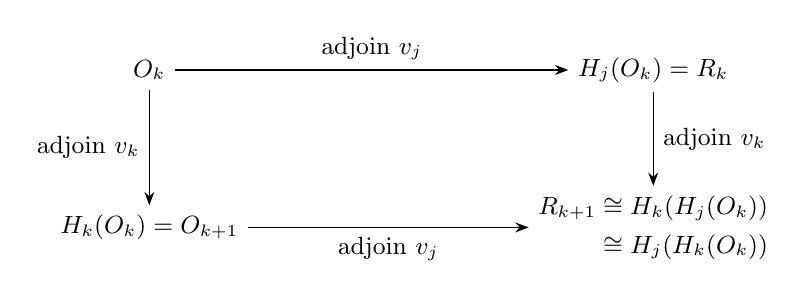
\begin{tikzpicture}[>=Stealth,every node/.style={font=\small}]
 \node (o) at (0,0) {$O_k$};
 \node (j) at (6.4,0) {$H_j(O_k)=R_k$};
 \node (k) at (0,-2) {$H_k(O_k)=O_{k+1}$};
 \node[align=center] (jk) at (6.4,-2)
 {$R_{k+1}\cong H_k(H_j(O_k))$\\[3pt]
  $\phantom{R_{k+1}}\cong H_j(H_k(O_k))$};
 \draw[->] (o) -- node[above] {adjoin $v_j$} (j);
 \draw[->] (o) -- node[left] {adjoin $v_k$} (k);
 \draw[->] (j) -- node[right] {adjoin $v_k$} (jk);
 \draw[->] (k) -- node[below] {adjoin $v_j$} (jk);
\end{tikzpicture}
\caption{Reordering two adjunctions whose data all lie in $O_k$.
The arrows are inclusions. Both paths give the same faithfully
tracial algebra, under an isomorphism fixing $O_k,v_j,v_k$.}
\label{fig:reordering}
\end{figure}

At a limit, the isomorphisms already constructed agree on overlaps
because they fix the named generators. The expectations from the
$O_\beta$ onto the two fixed abelian algebras generated by $(p_n)$
and $(q_n^j)$ also agree on overlaps, by
\cref{na:trace-expectation}. Applying \cref{na:hnn-limit} to these
fixed data identifies the closure of the preceding $H_j(O_\beta)$
with $H_j$ of the limit base, proving
\eqref{eq:omitted-adjunction} there.

At $\beta=\delta$ we have
$O_\delta=A[S\cup j]$ and
$R_\delta=A[S\cup(j+1)]$.
The two sequences still peak to inequivalent states on $O_\delta$,
by the first part of the proof. Thus \cref{na:bridge} applies to
\eqref{eq:omitted-adjunction}, giving \textup{(U)} for
\[
 A[S\cup j]\subset A[S\cup(j+1)].
\]
If $j\in S$ or $j$ is inactive, this inclusion is the identity.
The continuous chain $\bigl(A[S\cup j]\bigr)_{j\le\delta}$ starts
at $A[S]$ and ends at $X_\delta$; continuity follows because a
polynomial involves only finitely many indices outside $S$.
Now \cref{na:unique-chain} proves the theorem.
\end{proof}

\subsection{A separable algebra determines each pure state}

The separable pure-restriction argument below is closely related to
\cite[Proposition~2.3 and concluding Remark~1]{AkemannWassermannWeaver2010}.
Here we arrange that the separable algebra is dependency-closed;
\cref{na:closed-extension} then adds uniqueness of the full extension.

\begin{lemma}\label{na:countable-determination}
For every pure state $h$ of $X_\delta$, there is a countable
dependency-closed $S\subset\delta$ such that $h|_{A[S]}$ is pure
and $h$ is its unique state extension to $X_\delta$.
\end{lemma}
\begin{proof}
Construct increasing countable dependency-closed sets $S_n$, starting
with $S_0=\varnothing$. Choose a countable dense subset $D_n$ of
$A[S_n]$. For each $a\in D_n$ and each integer $m\ge1$,
\cref{na:excision} supplies a positive contraction $x_{a,m}$ in
$X_\delta$ satisfying
\[
 h(x_{a,m})=1,\qquad
 \bigl\|x_{a,m}(a-h(a)1)x_{a,m}\bigr\|<1/m.
\]
Each witness has countable support. Adjoin all these supports to
$S_n$ and close under dependencies to obtain $S_{n+1}$.

Set $S=\bigcup_n S_n$ and $B=A[S]$. Suppose
$h|_B=t h_1+(1-t)h_2$ for states $h_1,h_2$ and $0<t<1$.
Each $h_i$ takes value one on every witness $x_{a,m}$.
A positive contraction of state value one fixes the state's GNS
vector, so $h_i(a)=h_i(x_{a,m}a x_{a,m})$ and
$h_i(x_{a,m}^2)=1$. Hence
\[
 |h_i(a)-h(a)|
 =\bigl|h_i\bigl(x_{a,m}(a-h(a)1)x_{a,m}\bigr)\bigr|<1/m.
\]
Letting $m$ tend to infinity shows that both states agree with $h$
on every $D_n$. Their union is dense in $B$, so $h|_B$ is pure.
Its unique extension is $h$ by \cref{na:closed-extension}.
\end{proof}

\begin{corollary}\label{na:state-count}
Put $\mathfrak c=2^{\aleph_0}$. If $|\delta|\le\mathfrak c$, then
$X_\delta$ has at most $\mathfrak c$ pure states.
\end{corollary}
\begin{proof}
There are at most
\[
 \max(\aleph_0,|\delta|)^{\aleph_0}
 \le\mathfrak c^{\aleph_0}=\mathfrak c
\]
countable subsets of $\delta$. For each one, the corresponding
algebra $A[S]$ is separable and has at most $\mathfrak c$ states:
values on a countable dense subset determine a state. By
\cref{na:countable-determination}, every pure state of $X_\delta$
is the unique extension of one such restriction. There are at most
$\mathfrak c\cdot\mathfrak c=\mathfrak c$ possibilities.
\end{proof}

\section{The construction in ZFC}
\label{sec:construction}

We now choose the bridge steps so that every pure state eventually
joins the class of the state peaked by $(p_n)$. Countable
determination ensures that every pure state of the final algebra
will have appeared early enough to be treated.

\begin{theorem}[Kishimoto--Ozawa--Sakai]
\label{na:homogeneity}
Let $B$ be a separable $C^*$-algebra. If pure states $h,k$ of $B$
have GNS representations with the same kernel, there is an
automorphism $\gamma$ of $B$ such that $h\circ\gamma=k$.
In particular, this holds for every pair of pure states of a
separable simple $C^*$-algebra.
\end{theorem}

This is \cite[Theorem~1.1]{KishimotoOzawaSakai2003}, which in fact
provides an asymptotically inner automorphism. We apply it only to
the separable algebras $A[S]$ of \cref{na:inherited}.

\begin{proof}[Proof of \cref{na:main}]
Set $\kappa=\mathfrak c^+$. Every ordinal below $\kappa$ has
cardinality at most $\mathfrak c$, and every countable subset of
$\kappa$ is bounded: otherwise $\kappa$ would be a countable union
of sets of cardinality at most $\mathfrak c$, a contradiction.

\smallskip\noindent
\emph{Fix the schedule first.}
Before constructing any algebras, choose an injection
\begin{equation}\label{eq:schedule}
 \sigma:\kappa\times\kappa\longrightarrow\kappa,
 \qquad \sigma(\beta,\eta)\ge\beta.
\end{equation}
To do so, enumerate $\kappa\times\kappa$ in order type $\kappa$.
When a pair $(\beta,\eta)$ is encountered, choose an unused ordinal
at least $\beta$. Fewer than $\kappa$ ordinals have been used,
whereas the tail above $\beta$ has cardinality $\kappa$.
This defines the entire schedule without referring to any states.

\smallskip\noindent
\emph{Construct the algebras in ordinal order.}
Build a continuous bridge iteration $(X_\beta)_{\beta\le\kappa}$
starting from the algebra of \cref{na:base-peak}. For each
$\beta<\kappa$, once $X_\beta$ has been constructed, choose a list
\[
 (h_{\beta,\eta})_{\eta<\kappa}
\]
containing every pure state of $X_\beta$, with repetitions allowed.
This is possible by \cref{na:state-count}, since
$|\beta|\le\mathfrak c$ for $\beta<\kappa$.

At stage $j<\kappa$, let $f$ be the state of $X_j$ peaked by
$(p_n)$. If $j$ is outside the range of $\sigma$, make the identity
step. Otherwise write $j=\sigma(\beta,\eta)$ and let $g$ be the
unique lift of $h_{\beta,\eta}$ to $X_j$. The list for $\beta$ is
already available because $\beta\le j$; when $\beta=j$, it is
chosen before the successor step. If $g\sim f$, again make the
identity step.

Suppose $g\not\sim f$. By \cref{na:countable-determination}, choose
a countable dependency-closed $S\subset j$ such that $g|_{A[S]}$
is pure and uniquely determines $g$ on $X_j$. The restriction
$f|_{A[S]}$ is pure by \cref{na:peaking-restriction}. The algebra
$A[S]$ is separable, simple and unital by \cref{na:inherited}.
Applying \cref{na:homogeneity}, choose an automorphism $\gamma$
of $A[S]$ with
\[
 (g|_{A[S]})\circ\gamma=f|_{A[S]},
 \qquad q_n^j=\gamma(p_n)\quad(n\ge0).
\]
If a state on $A[S]$ takes value one on every $q_n^j$, composing
it with $\gamma$ gives the unique state taking value one on every
$p_n$. Thus $(q_n^j)$ peaks to $g|_{A[S]}$. By
\cref{na:closed-extension}, it peaks to $g$ on $X_j$ as well.

The trace requirement deserves a separate check. For each $n$,
$\gamma$ carries the unital matrix stage $M_{2^n}\subset A_0$
onto a unital matrix subalgebra of $A[S]$, and carries its minimal
projection $p_n$ to $q_n^j$. The ambient trace restricts to the
unique normalized trace on this matrix algebra. Consequently,
\[
 \tau(q_n^j)=2^{-n}=\tau(p_n).
\]
This argument does not require an automorphism to preserve the
specified trace on all of $A[S]$.

We can therefore perform the bridge of \cref{na:bridge} with
$(p_n),(q_n^j)$, and set $I_j=S$. At an identity step set
$I_j=\varnothing$. At limit stages take the norm completion of
the union. Each successor satisfies \textup{(U)} and has a faithful
trace-preserving expectation onto its base. The results of
\cref{sec:iteration} therefore apply throughout the recursion.

All choices are set-sized. At every stage the algebra is generated
by at most $\kappa$ elements, so its density is at most $\kappa$
and its underlying cardinality at most $\lambda=\kappa^{\aleph_0}$.
Fix a set of cardinality $\lambda$. Algebra structures on its
subsets, together with their norms, traces, embeddings, states,
automorphisms and lists, form a set of codes. Well-order that set
to make the required choices; recode successor algebras with their
embeddings and use norm inductive limits. Ordinary choice and
transfinite recursion in ZFC suffice.

\smallskip\noindent
\emph{Every final pure state is treated.}
Let $A=X_\kappa$ and let $h$ be any pure state of $A$.
By \cref{na:countable-determination}, there is a countable
dependency-closed $S\subset\kappa$ such that $h|_{A[S]}$ is pure
and has unique extension $h$ to $A$. Boundedness of $S$ gives
$\beta<\kappa$ with $A[S]\subset X_\beta$.
The state $h|_{X_\beta}$ is the unique extension of $h|_{A[S]}$
to $X_\beta$: any other extension could itself be extended to
$A$, contradicting uniqueness there. Hence $h|_{X_\beta}$ is pure.

Choose $\eta$ with $h_{\beta,\eta}=h|_{X_\beta}$ and put
$j=\sigma(\beta,\eta)$. Its lift to $X_j$ is $h|_{X_j}$.
At stage $j$ this lift either already belongs to the $p_n$-class
or is joined to it by the bridge. By \cref{na:unique-chain}, the
equivalence persists to $A$. Thus all pure states of $A$ have
unitarily equivalent GNS representations.

Every nonzero irreducible representation $\pi$ of the unital
algebra $A$ is unital: the range of $\pi(1)$ is a nonzero closed
invariant subspace. Every nonzero vector is cyclic by irreducibility,
so each unit vector defines a pure state whose GNS representation
is equivalent to $\pi$. The $p_n$-state supplies one such
representation. Therefore $A$ has exactly one nonzero irreducible
representation up to unitary equivalence.

Finally, $A$ is simple and has a faithful tracial state by
\cref{na:inherited} and the limit permanence facts. It is unital
and contains the infinite-dimensional algebra $A_0$. An algebra
$K(H)$ is unital only when $H$ is finite-dimensional:
the identity on an infinite-dimensional Hilbert space is not
compact, as an infinite orthonormal sequence has no norm-convergent
subsequence. The finite-dimensional case, including $H=0$, cannot
be isomorphic to $A$. This proves the theorem.
\end{proof}

{\small
\bibliographystyle{plain}
\bibliography{references}
}
\end{document}
